%%%%%%%%%%%%%%%%%%%%%%%%%%%%%%%%%%%%%%%%%%%%%%%%%%%%%%%%%%%%%%%%%%%%%%%%%%%%%%%
\section{A Single-Step Framework for MGXS Generation}
\label{sec:single-step}
%%%%%%%%%%%%%%%%%%%%%%%%%%%%%%%%%%%%%%%%%%%%%%%%%%%%%%%%%%%%%%%%%%%%%%%%%%%%%%%

In general, MGXS generation schemes use a multi-step approach to decouple the energy, angular and spatial dimensions of the transport equation. The multi-step approach typically applies high-fidelity models of the energy self-shielding physics to low-fidelity geometric models of unique core components as illustrated in \autoref{fig:multi-step-framework}. The multi-step approach uses a combination of models of varying complexity to optimize overall simulation speed with accuracy. However, this is often done at the expense of generality. For example, multi-step MGXS generation schemes do not typically model inter-assembly physics or the effect of reflectors and other core heterogeneities on the spatial distribution of the flux. The approximations to the energy and spatial variation of the flux introduce approximation error in full-core calculations and limit the core design parameter space for which multi-step schemes may be applied. 

\begin{figure}[h!]
\centering
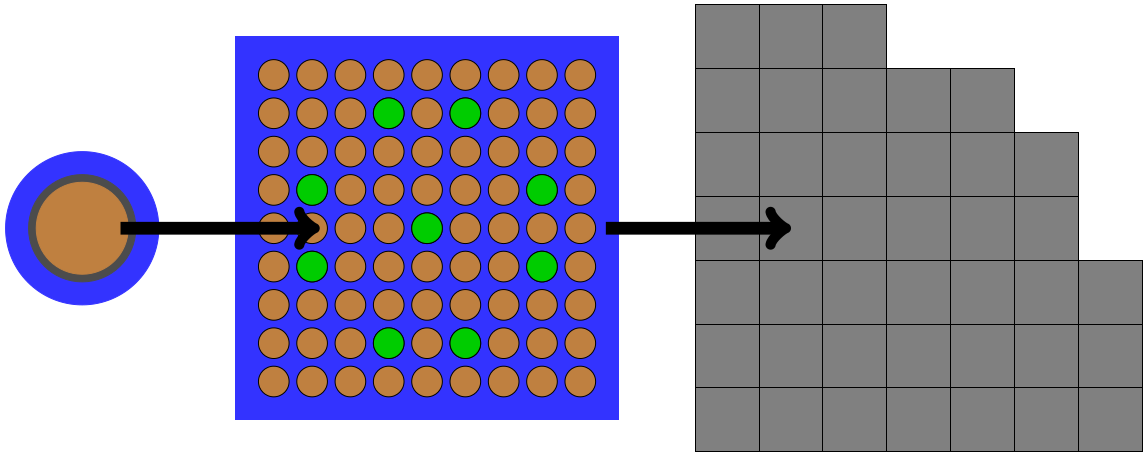
\includegraphics[width=0.8\linewidth]{figures/multi-step-flow-chart}
\caption{The multi-step approach typically used for multi-group reactor physics calculations \cite{gibson2016thesis}.}
\label{fig:multi-step-framework}
\end{figure}

Monte Carlo-based MGXS generation methods to date have retained the multi-step geometric framework to tabulate MGXS for individual reactor components -- such as infinite fuel pins and/or assemblies -- for subsequent use in full-core multi-group calculations. Indeed, the \texttt{openmc.mgxs} module can be configured within a multi-step framework to generate MGXS for infinite fuel pins or assemblies. Although the use of MC within a multi-step framework eliminates the need to approximate the flux in energy, it does not account for spatial self-shielding effects throughout a reactor core. Alternatively, the \texttt{openmc.mgxs} module may be configured in a novel single-step framework that uses OpenMC eigenvalue simulations of the complete heterogeneous geometry to simultaneously account for all energy and spatial effects in a single step. The single-step framework permits a rigorous quantification of approximation error due to energy and spatial self-shielding models used by deterministic methods for MGXS generation. Both single-step and multi-step frameworks are evaluated for two heterogeneous PWR benchmarks in the following sections.

%may be impractical for MGXS generation for industrial applications since it is constrained by the slow convergence rate of Monte Carlo tallies. Nevertheless, it allows for the


%%%%%%%%%%%%%%%%%%%%%%%%%%%%%%%%%%%%%%%%%%%%%%%%%%%%%%%%%%%%
\subsection{MGXS Generation with OpenMC}
\label{subsec:openmc}

OpenMC was employed to generate MGXS, and reference eigenvalues and pin-wise fission and U-238 capture rates. The MGXS were tallied in CASMO's seventy energy group structure \cite{rhodes2006casmo}. The OpenMC simulations were performed with 1000 batches with 10$^{6}$ particle histories per batch. Stationarity of the fission source was obtained with 100 inactive batches for both benchmarks. The OpenMC simulations used the ``iso-in-lab'' feature to enforce isotropic in lab scattering. The ``iso-in-lab'' feature samples the outgoing neutron energy from the scattering laws prescribed by the continuous energy cross section library, but the outgoing neutron direction of motion is sampled from an isotropic in lab distribution. Although isotropic in lab scattering is a poor approximation for LWRs, it eliminated scattering source anisotropy as one possible cause of approximation error between OpenMC and OpenMOC. 

The \textit{multi-step} framework employs multiple OpenMC simulations to compute MGXS for each heterogeneous benchmark. In particular, the MGXS are generated by OpenMC simulations of each unique fuel pin type (\textit{e.g.}, enrichment) in an infinite, repeating array\footnote{An infinite, repeating array of fuel pins is modeled by a single fuel pin with reflective boundary conditions.}. The \textit{single-step} framework uses a single OpenMC eigenvalue calculation of the complete heterogeneous geometry to generate MGXS for each material. The spatially self-shielded flux is used to collapse the cross sections in each material with a unique isotopic composition. The null scheme does not account for spatial self-shielding effects experienced by different fuel pins filled by the same fuel composition, and instead averages these effects across the entire geometry. A single MGXS is employed in each instance of a material zone, such as a fuel pin replicated many times throughout a benchmark geometry. The multi-step and single-step frameworks can be compared to quantify the impact of using the ``true'' Monte Carlo flux from an infinite lattice calculation, rather than the ``true'' MC flux from the true heterogeneous geometry, to collapse MGXS for each type of material. 


%%%%%%%%%%%%%%%%%%%%%%%%%%%%%%%%%%%%%%%%%%%%%%%%%%%%%%%%%%%%
\subsection{Multi-Group Calculations with OpenMOC}
\label{subsec:openmoc}

The OpenMOC code \cite{boyd2014openmoc} was employed to use the MGXS generated by OpenMC for deterministic multi-group transport calculations. The OpenMOC code is a 2D method of characteristics code designed for fixed source and eigenvalue neutron transport calculations. OpenMOC approximates the scattering source as isotropic in the lab coordinate system, and discretizes the geometry into flat source regions (FSRs) which approximate the neutron source as constant across each spatial zone. The OpenMOC eigenvalue and energy-integrated, pin-wise reaction rates were compared with the reference solutions computed by OpenMC. Each OpenMOC simulation used a characteristic track laydown with 128 azimuthal angles and 0.05 cm spacing, and was converged to 10$^{-5}$ on the root mean square of the energy-integrated fission source in each FSR. Coarse Mesh Finite Difference acceleration was applied on a pin-wise spatial mesh to reduce the number of iterations required to converge the fine-mesh transport calculations.


%%%%%%%%%%%%%%%%%%%%%%%%%%%%%%%%%%%%%%%%%%%%%
\subsection{Benchmarks and Reference Results}
\label{subsec:benchmarks}

This paper modeled benchmarks derived from the Benchmark for Evaluation And Validation of Reactor Simulations (BEAVRS) PWR model~\cite{horelik2013beavrs}. Each test case includes heterogeneous features -- and corresponding spatial self-shielding effects -- to demonstrate the potential utility of a single-step framework for MGXS generation. The benchmarks were comprised of materials from the BEAVRS model, including 1.6\% and 3.1\% enriched UO$_2$ fuel, borated water (975 ppm boron), zircaloy, helium, air, borosilicate glass and stainless steel. Each material was modeled with cross sections from the ENDF/B-VII.1 continuous energy cross section library~\cite{mcnpx2003manual} evaluated at 600K for hot zero power conditions. 

%Although BEAVRS is an axially heterogeneous 3D core model, both benchmarks were fabricated in 2D due to the geometric constraints in OpenMOC.

The first benchmark was a single fuel assembly with an array of 264 fuel pins of 1.6\% enriched UO$_2$ fuel with zircaloy cladding and a helium gap. The assembly included 24 control rod guide tubes (CRGTs) filled by borated water and surrounded by zircaloy cladding, and a central instrument tube filled with air surrounded by two zircaloy tubes separated by borated water. The second benchmark was constructed as a 2$\times$2 colorset of two fuel assemblies extracted from the BEAVRS model. The top-left and bottom-right fuel assemblies were of the same enrichment and configuration as the single assembly benchmark. The top-right and bottom-left fuel assemblies included 264 fuel pins of 3.1\% enriched UO$_2$ fuel, 20 CRGTs and a central instrument tube. In addition, the two 3.1\% enriched assemblies included four burnable poisons (BPs) consisting of eight layers of air, steel, borosilicate glass and zircaloy. The colorset was surrounded by a water reflector on the bottom and right that was of the same width as a fuel assembly. The assembly benchmark was modeled with reflective boundary conditions, while the colorset was modeled with reflective boundaries on the top and left and vacuum boundaries on the bottom and right. The assembly and colorset are illustrated in \autoref{fig:benchmarks-materials}.

%The intra-pin grid spacers and grid sleeves separating each assembly in the BEAVRS model were not included either benchmark. 

\begin{figure}[h!]
\centering
\begin{subfigure}{0.42\textwidth}
  \centering
  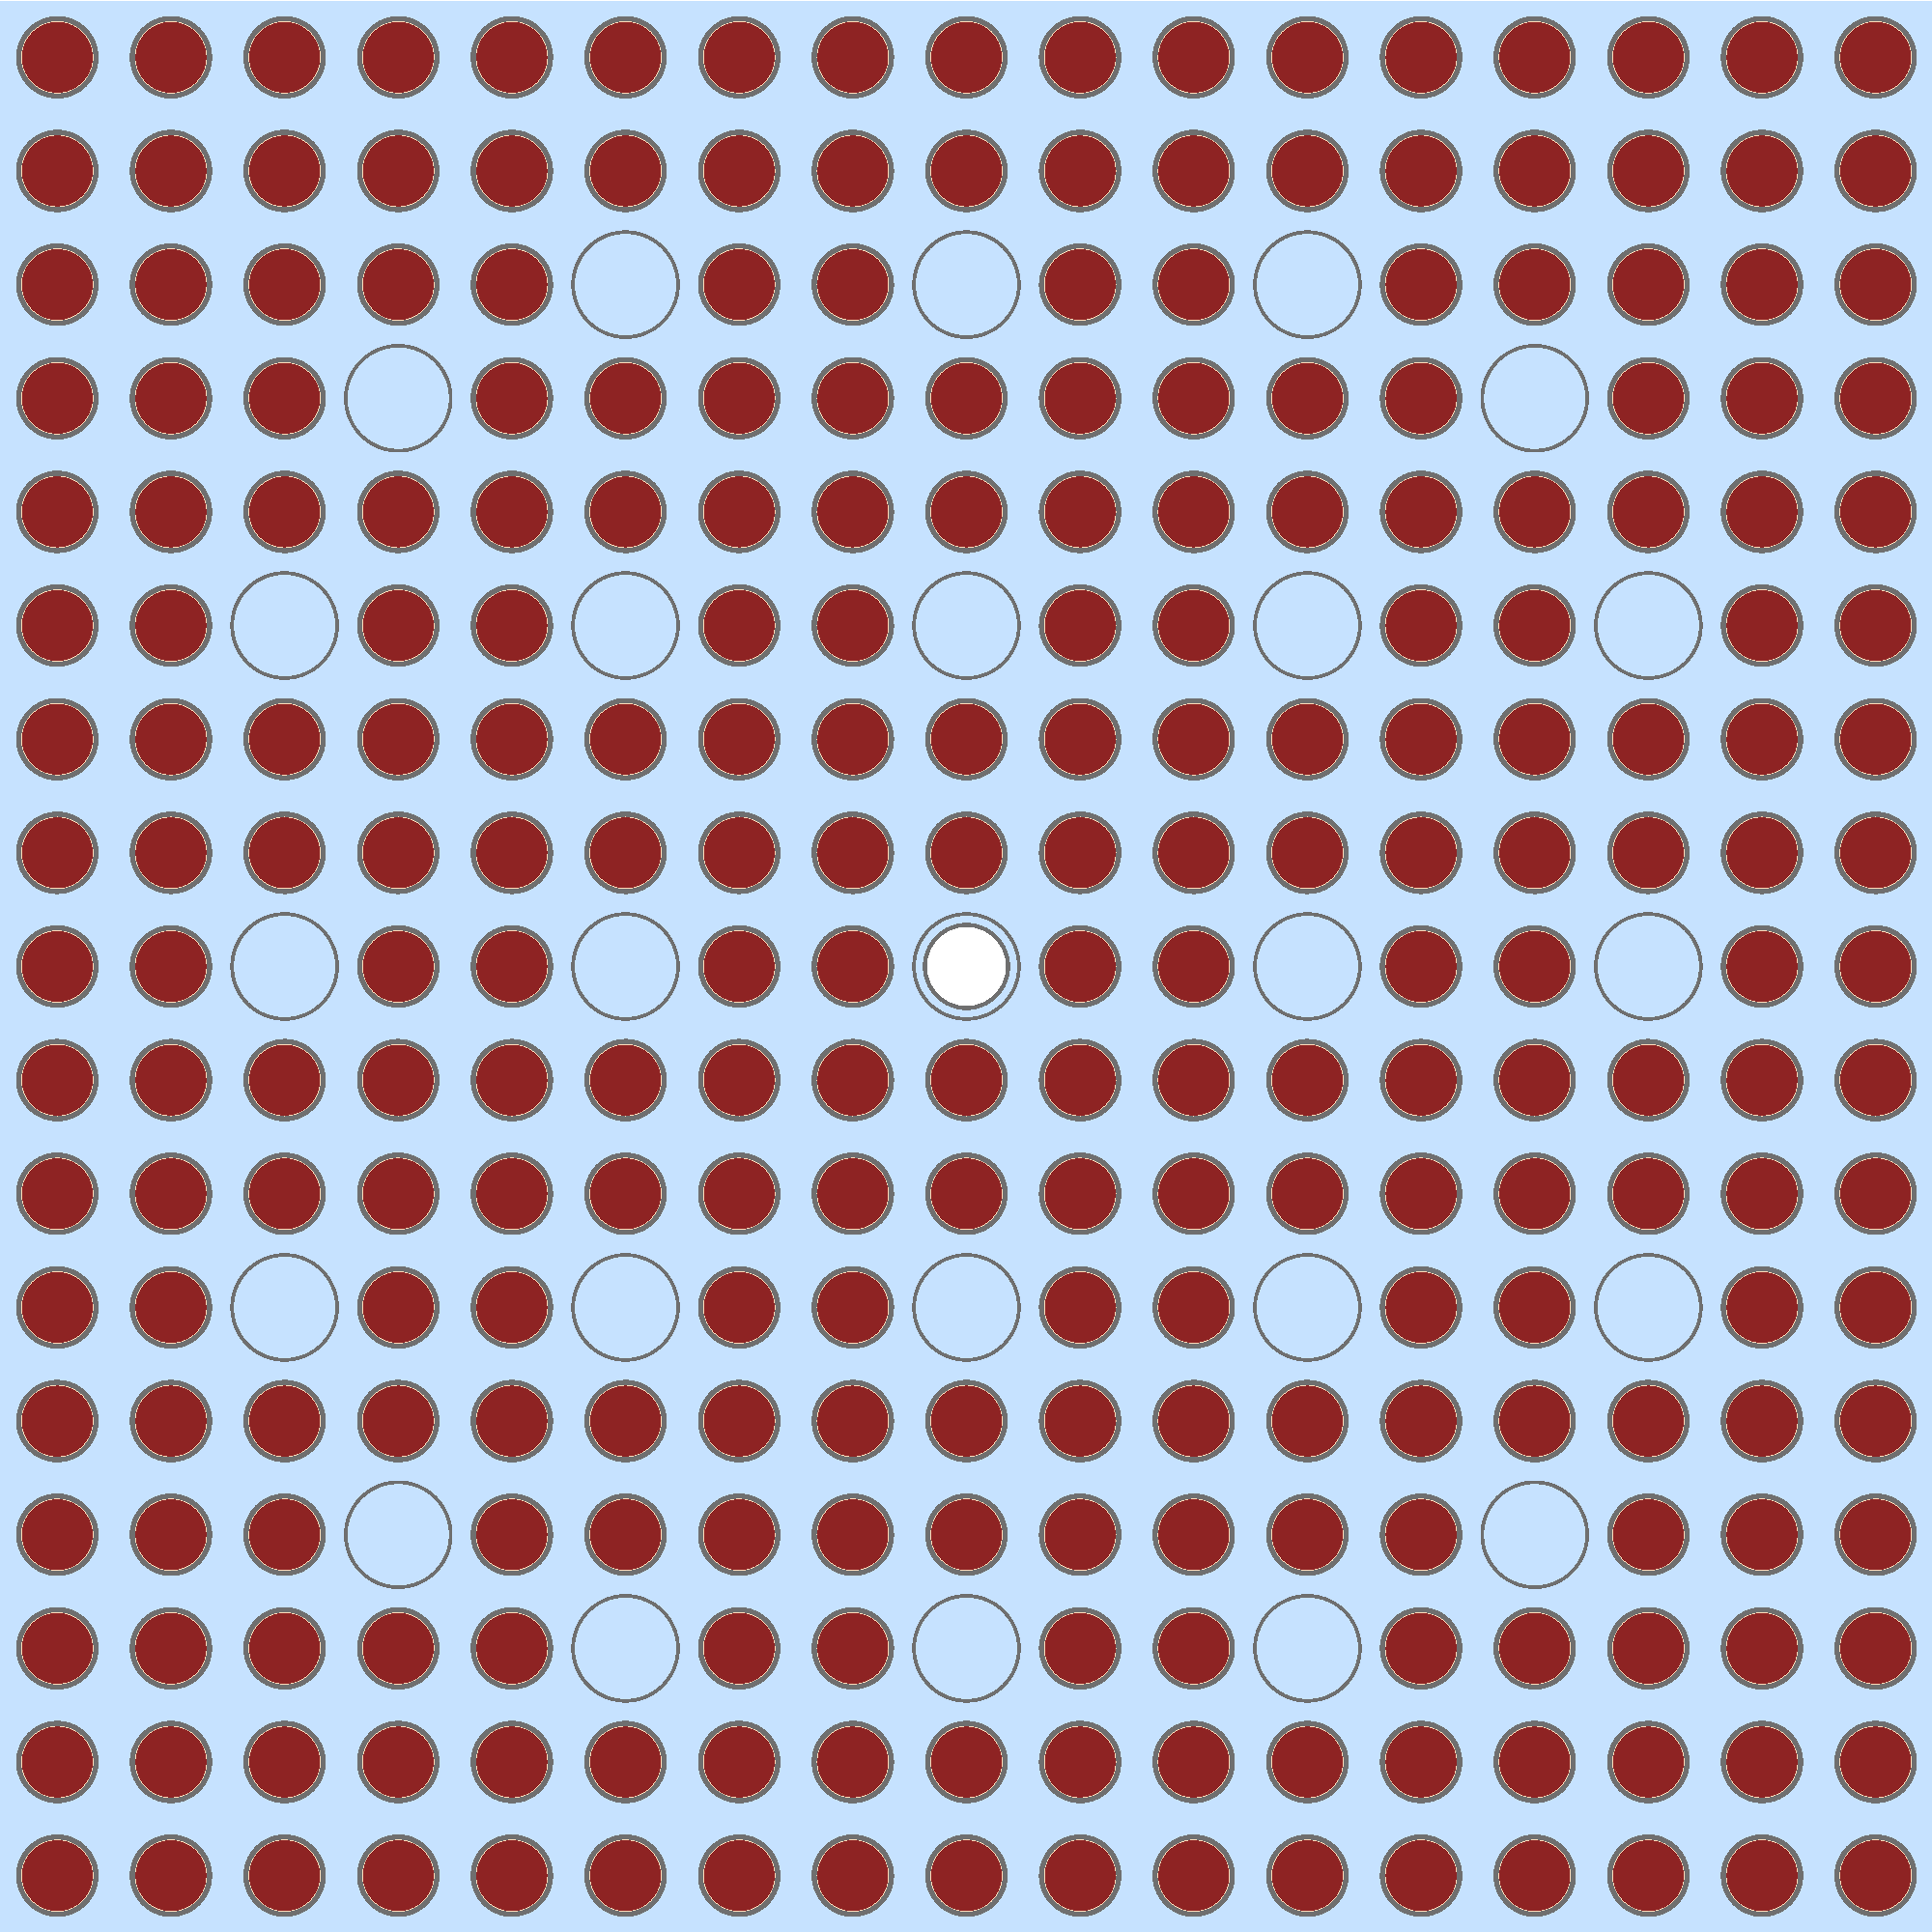
\includegraphics[width=0.8\linewidth]{figures/assembly/geometry}
  \caption{}
  \label{fig:benchmarks}
\end{subfigure}
\begin{subfigure}{0.42\textwidth}
  \centering
  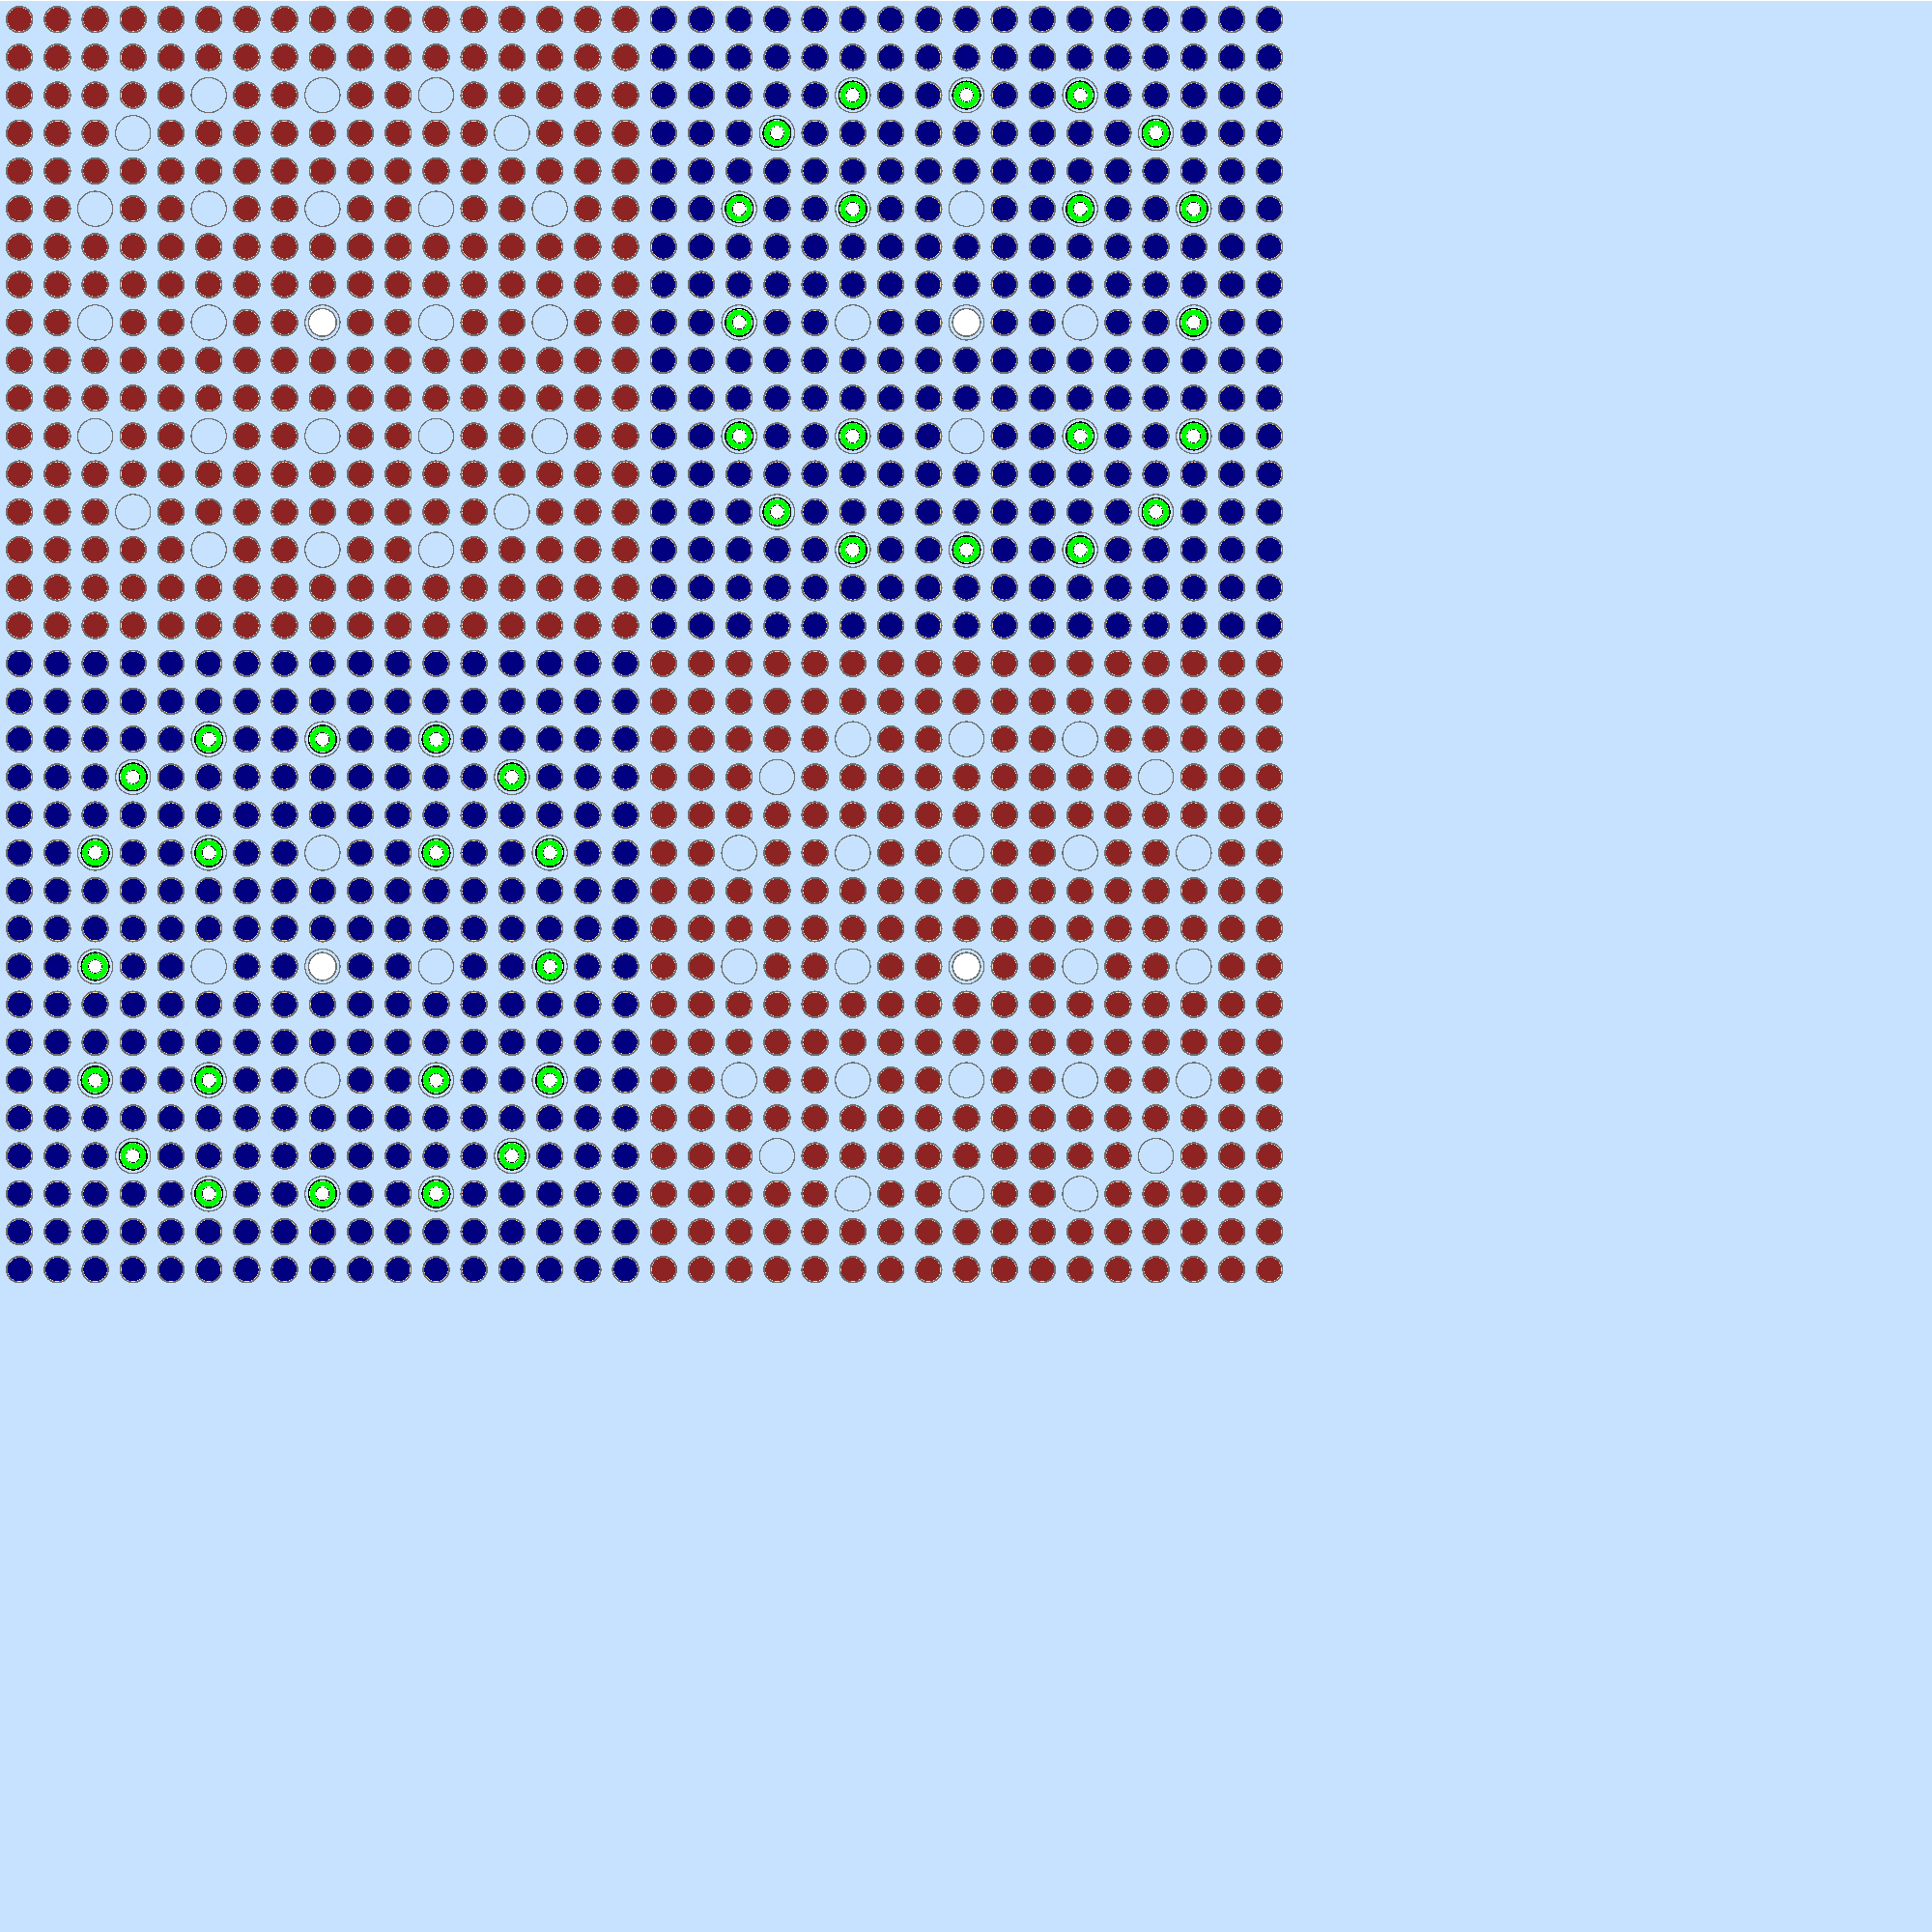
\includegraphics[width=0.8\linewidth]{figures/colorset/geometry}
  \caption{}
  \label{fig:benchmarks-colorset}
\end{subfigure}
\caption{The assembly (a) and colorset (b) benchmark geometries.}
\label{fig:benchmarks-materials}
\end{figure}

\begin{figure}[h!]
\centering
\begin{subfigure}{0.42\textwidth}
  \centering
  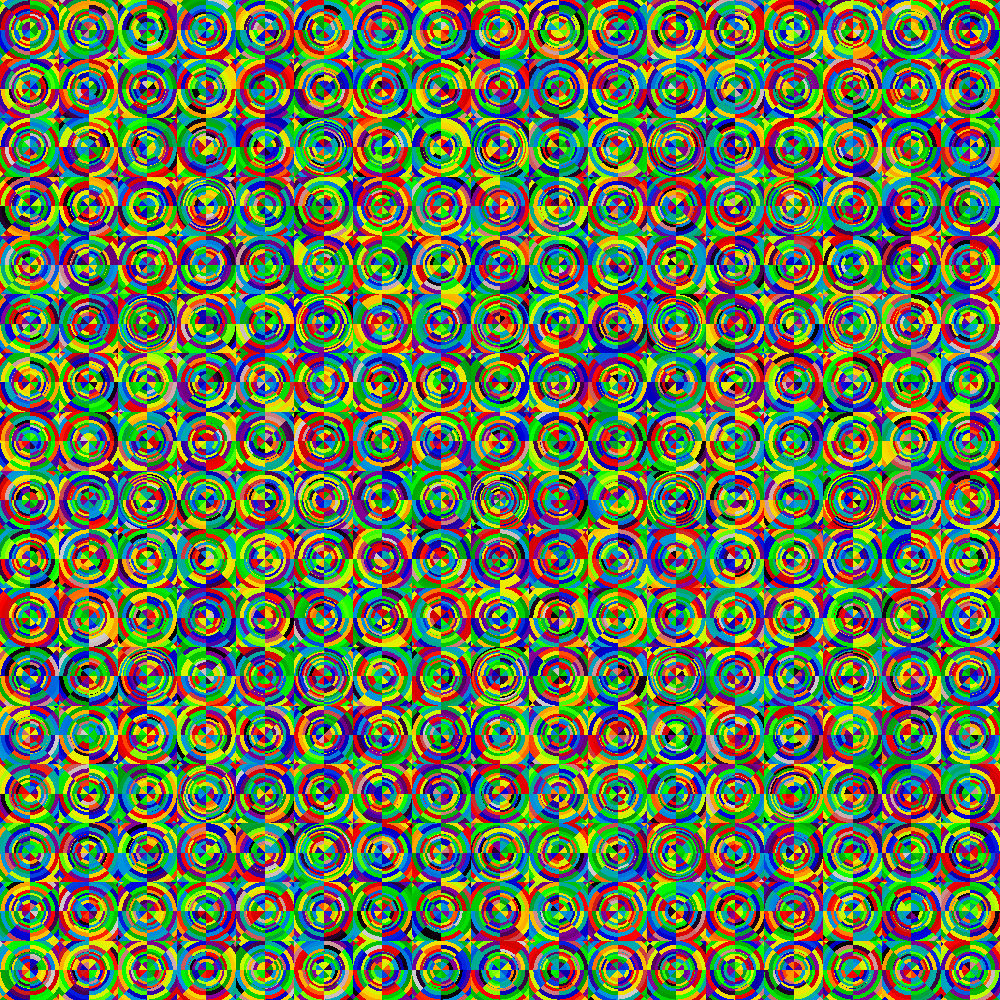
\includegraphics[width=0.8\linewidth]{figures/assembly/fsrs}
  \caption{}
  \label{fig:benchmarks-assm-fsrs}
\end{subfigure}%
\begin{subfigure}{0.42\textwidth}
  \centering
  
\includegraphics[width=0.8\linewidth]{figures/colorset/fsrs}
  \caption{}
  \label{fig:benchmarks-colorset-fsrs}
\end{subfigure}
\caption{OpenMOC flat source regions for the assembly (a) and colorset (b) benchmarks.}
\label{fig:benchmarks-fsrs}
\end{figure}

Flat source region spatial discretization meshes were applied to both benchmarks for the OpenMOC simulations as shown in \autoref{fig:benchmarks-fsrs}. The UO$_2$ fuel was subdivided into five equal volume radial rings, while ten radial rings were employed in the water-filled CRGTs and instrument tubes. The borosilicate glass and borated water material zones filling the BPs were each discretized into five equal volume radial rings. Five equally spaced rings were used in the moderator zones surrounding each pin. Eight equal angle subdivisions were used in all pin cell material zones. The 13.85824 cm of water reflector nearest the fuel assemblies in the colorset benchmark was discretized in a 0.125984 cm $\times$ 0.125984 cm rectilinear mesh, equivalent to a 10$\times$10 mesh in each pin. The 7.55904 cm of reflector furthest from the fuel assemblies was discretized in a 1.25984 cm $\times$ 1.25984 cm pin-wise mesh.

A series of OpenMC simulations was used to calculate reference eigenvalues, pin-wise fission rates, and pin-wise U-238 capture rates for both benchmarks. The reference solutions were computed with 100 inactive and 900 active batches of 10$^7$ particle histories per batch. The OpenMC ``combined'' eigenvalue estimator is reported along with the associated 1-sigma uncertainty of one pcm for both benchmarks in \autoref{tab:keff-reference}. The reference energy-integrated fission and U-238 capture rate spatial distributions were computed using rectilinear, pin-wise tally meshes in OpenMC and are shown in \autoref{fig:benchmarks-rxn-rates}. The reaction rates were normalized to the mean of all non-zero reaction rates. The rates in the instrument tubes, CRGTs and BPs are all zero and are shaded in white. The 1-sigma uncertainties are less than 0.08\% in each pin for both benchmarks.

\begin{table}[h!]
  \centering
  \caption{Reference OpenMC eigenvalues for each benchmark.}
  \label{tab:keff-reference} 
  \begin{tabular}{c c}
  \toprule
  {\bf Assembly} &
  {\bf Colorset} \\
  \midrule
  0.99326 $\pm$ 0.00001 & 0.94574 $\pm$ 0.00001 \\
  \bottomrule
\end{tabular}
\end{table}

\begin{figure*}[h!]
\centering
\begin{subfigure}{0.45\textwidth}
  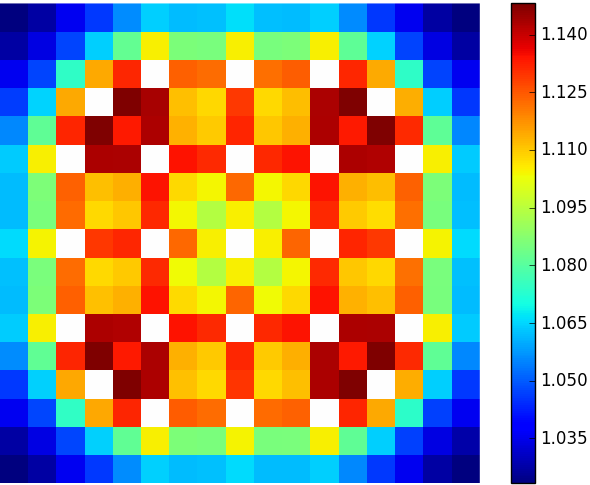
\includegraphics[width=\linewidth]{figures/assembly/fission-rates}
  \caption{}
  \label{fig:fiss-assm}
\end{subfigure}%
\begin{subfigure}{0.45\textwidth}
  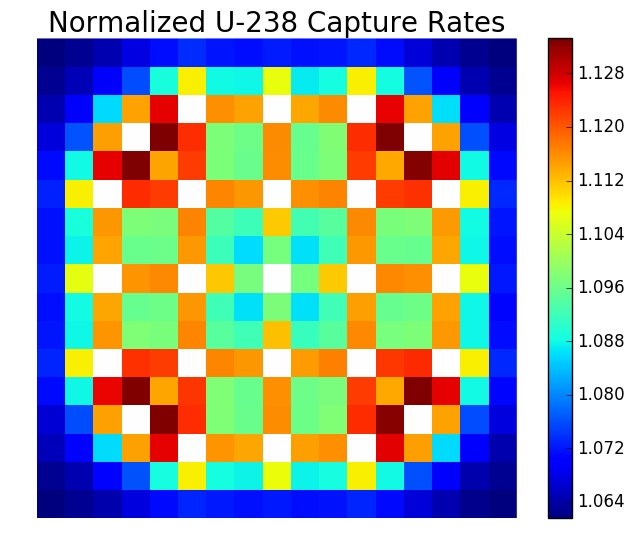
\includegraphics[width=\linewidth]{figures/assembly/capture-rates}
  \caption{}
  \label{fig:capt-assm}
\end{subfigure}
\begin{subfigure}{0.45\textwidth}
  \centering
  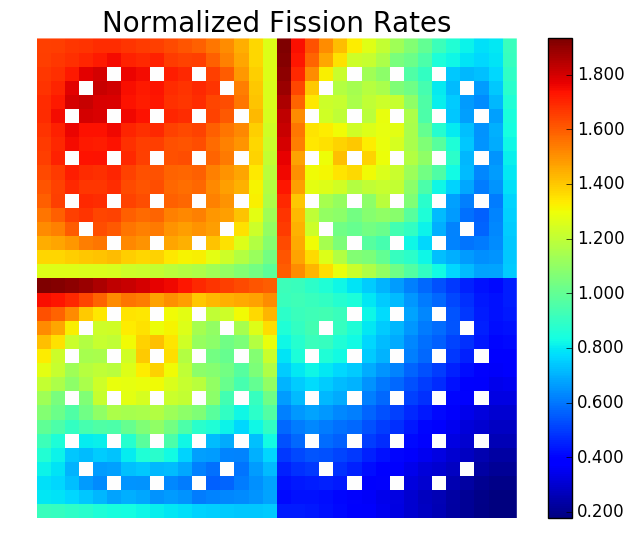
\includegraphics[width=\linewidth]{figures/colorset/fission-rates}
  \caption{}
  \label{fig:fiss-colorset}
\end{subfigure}%
\begin{subfigure}{0.45\textwidth}
  \centering
  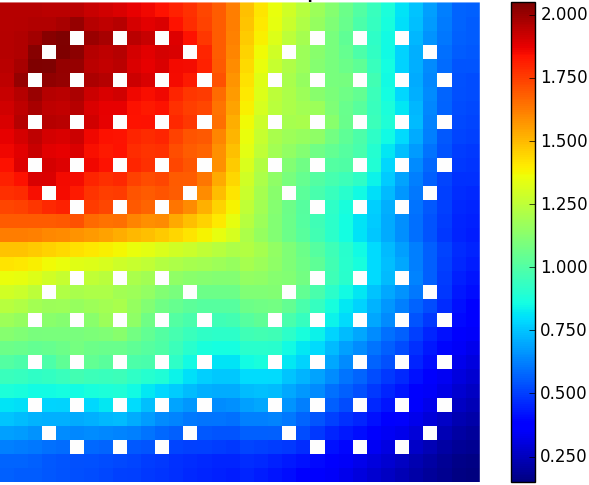
\includegraphics[width=\linewidth]{figures/colorset/capture-rates}
  \caption{}
  \label{fig:capt-colorset}
\end{subfigure}
\caption{Reference OpenMC fission and U-238 capture rates for the assembly (a) -- (b) and colorset (c) -- (d) benchmarks.}
\label{fig:benchmarks-rxn-rates}
\end{figure*}


%%%%%%%%%%%%%%%%%%%%%%%%%%%%%%%%%%%%%%%%%%%%%%%%%%%%%%%%%%%%%%%%%%%%%%%%%%%%%%%
\subsection{Results}
\label{subsec:results}
%%%%%%%%%%%%%%%%%%%%%%%%%%%%%%%%%%%%%%%%%%%%%%%%%%%%%%%%%%%%%%%%%%%%%%%%%%%%%%%

Both benchmarks were modeled with OpenMOC using MGXS generated by OpenMC using the single-step framework. The OpenMOC eigenvalues were compared to the reference OpenMC eigenvalues from \autoref{tab:keff-reference}. The eigenvalue bias $\Delta\rho$ was calculated by comparing the eigenvalue $k_{eff}^{MOC}$ from OpenMOC to the reference eigenvalue $k_{eff}^{MC}$ computed by OpenMC in units of per cent mille (pcm):

\begin{equation}
\label{eqn:delta-rho}
\Delta\rho = \left(k_{eff}^{MOC} - k_{eff}^{MC}\right) \times 10^{5}
\end{equation}

The bias is listed for both benchmarks in \autoref{tab:keff-bias}. The slightly negative bias of a few hundred pcm is likely due to the flux separability approximation \cite{boyd2017sph}, which permits use of the scalar rather than the angular neutron flux to collapse cross sections. 

%It should be recalled that isotropic in lab scattering is used by OpenMC to compute both the reference solution and the MGXS. If anisotropic scattering were employed in OpenMC, one would expect quite different biases without a robust implementation of a higher order scattering kernel in OpenMOC.

\begin{table}[h!]
  \centering
  \caption{OpenMOC eigenvalue bias $\Delta\rho$.}
  \label{tab:keff-bias} 
  \begin{tabular}{l l r r r}
  \toprule
  \textbf{Benchmark} & \textbf{MGXS Scheme} & \textbf{2-Group} & \textbf{8-Group} & \textbf{70-Group} \\
  \midrule
  \multirow{2}{*}{Assembly} & Multi-Step    & -132 & -68 &   31 \\
                            & Single-Step &   60 & -72 & -161 \\
  \midrule
  \multirow{2}{*}{Colorset} & Multi-Step    & 2103 & 267 &   46 \\
                            & Single-Step & 1818 & 478 & -142 \\
  \bottomrule
\end{tabular}
\end{table}

The OpenMOC energy-integrated pin-wise fission rates were compared to the reference OpenMC fission rates \autoref{fig:benchmarks-rxn-rates}. The percent relative errors for each pin's fission rates were computed and the maximum and mean errors are listed in \autoref{tab:fiss-max-errors} and \autoref{tab:fiss-mean-errors}, respectively. In particular, the maximum errors are the maximum of the absolute values of the errors along with the appropriate sign, while the mean errors are the averages of the absolute error magnitudes.

\begin{table}[h!]
  \centering
  \caption{OpenMOC maximum fission rate percent relative errors.}
  \label{tab:fiss-max-errors}
  \begin{tabular}{l l c c c}
  \toprule
  \textbf{Benchmark} & \textbf{MGXS Scheme} & \textbf{2-Group} & \textbf{8-Group} & \textbf{70-Group} \\
  \midrule
  \multirow{2}{*}{Assembly} & Multi-Step    & 2.387 & 0.643 & 0.375 \\
                            & Single-Step & 2.379 & 0.638 & 0.380 \\
  \midrule
  \multirow{2}{*}{Colorset} & Multi-Step    &  11.024 &  2.773 & 0.670 \\
                            & Single-Step & -16.330 & -2.855 & 0.764 \\
  \bottomrule
\end{tabular}
\end{table}

\begin{table}[h!]
  \centering
  \caption{OpenMOC mean absolute fission rate percent relative errors.}
  \label{tab:fiss-mean-errors}
  \begin{tabular}{l l c c c}
  \toprule
  \textbf{Benchmark} & \textbf{MGXS Scheme} & \textbf{2-Group} & \textbf{8-Group} & \textbf{70-Group} \\
  \midrule
  \multirow{2}{*}{Assembly} & Multi-Step    & 0.951 & 0.231 & 0.073 \\
                            & Single-Step & 0.943 & 0.229 & 0.074 \\
  \midrule
  \multirow{2}{*}{Colorset} & Multi-Step    & 4.964 & 1.029 & 0.147 \\
                            & Single-Step & 5.471 & 1.080 & 0.178 \\
  \bottomrule
\end{tabular}
\end{table}

The spatial distributions of fission rate errors for the single-step framework are plotted as heatmaps for each benchmark in \autoref{fig:fiss-errors}. The heatmaps illustrate systematic trends in the pin-wise fission errors which correlate with spatial heterogeneities in each benchmark. In particular, the fission rates are generally underpredicted for pins adjacent to a single CRGT, but overpredicted for pins adjacent to two CRGTs in the assembly. In addition, the errors are largest for pins along the inter-assembly and assembly-reflector interfaces for the colorset benchmark.

%For the PWR benchmarks modeled here, the moderation provided by neighboring CRGTs and reflectors softens the flux for nearby fuel pins and should be modeled when collapsing pin-wise MGXS for high-fidelity multi-group transport calculations.

\begin{figure*}[h!]
\centering
\begin{subfigure}{0.45\textwidth}
  \centering
  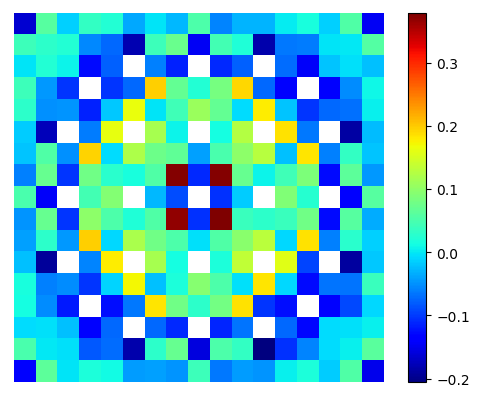
\includegraphics[width=\linewidth]{figures/assembly/fiss-single-step-errors}
  \caption{}
  \label{fig:assm-fiss-single-step-error}
\end{subfigure}%
\begin{subfigure}{0.45\textwidth}
  \centering
  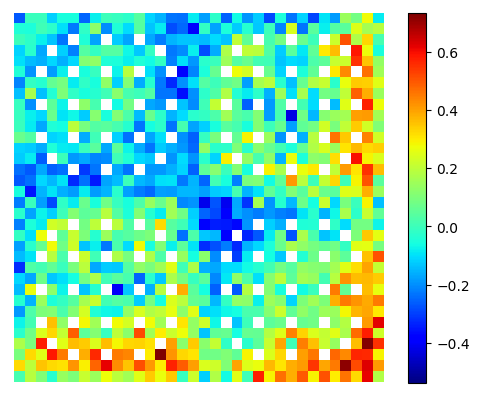
\includegraphics[width=\linewidth]{figures/colorset/fiss-single-step-errors}
  \caption{}
  \label{fig:colorset-fiss-single-step-error}
\end{subfigure}
\caption{OpenMOC fission rate percent relative errors for the assembly (a) and colorset (b) benchmarks.}
\label{fig:fiss-errors}
\end{figure*}

The OpenMOC energy-integrated pin-wise U-238 capture rates were compared to the reference OpenMC capture rates shown in \autoref{fig:benchmarks-rxn-rates}. The percent relative errors for each pin's capture rates were computed and the maximum and mean errors are listed in \autoref{tab:capt-max-errors} and \autoref{tab:capt-mean-errors}, respectively. In particular, the maximum errors are the maximum of the absolute values of the errors along with the appropriate sign, while the mean errors are the averages of the absolute error magnitudes.

\begin{table}[h!]
  \centering
  \caption{OpenMOC maximum U-238 capture rate percent relative errors.}
  \label{tab:capt-max-errors}
  \begin{tabular}{l l c c c}
  \toprule
  \textbf{Benchmark} & \textbf{MGXS Scheme} & \textbf{2-Group} & \textbf{8-Group} & \textbf{70-Group} \\
  \midrule
  \multirow{2}{*}{Assembly} & Multi-Step    & -2.644 & -1.480 & -1.102 \\
                            & Single-Step & -2.629 & -1.475 & -1.101 \\
  \midrule
  \multirow{2}{*}{Colorset} & Multi-Step    & 12.010 & 3.618 & -1.889 \\
                            & Single-Step & 11.100 & 3.372 & -1.969 \\
  \bottomrule
\end{tabular}
\end{table}

\begin{table}[h!]
  \centering
  \caption{OpenMOC mean absolute U-238 capture rate percent relative errors.}
  \label{tab:capt-mean-errors}
  \begin{tabular}{l l c c c}
  \toprule
  \textbf{Benchmark} & \textbf{MGXS Scheme} & \textbf{2-Group} & \textbf{8-Group} & \textbf{70-Group} \\
  \midrule
  \multirow{2}{*}{Assembly} & Multi-Step    & 1.252 & 0.643 & 0.480 \\
                            & Single-Step & 1.247 & 0.641 & 0.479 \\
  \midrule
  \multirow{2}{*}{Colorset} & Multi-Step    & 3.878 & 0.847 & 0.480 \\
                            & Single-Step & 3.708 & 0.780 & 0.478 \\
  \bottomrule
\end{tabular}
\end{table}

The spatial distributions of capture rate errors are plotted as heatmaps for each benchmark in \autoref{fig:capt-errors}. The heatmaps illustrate systematic error trends in the pin-wise capture errors which correlate with spatial heterogeneities in each benchmark. This underscores the importance of accounting for spatial heterogeneities -- such as the added moderation from CRGTs and reflectors -- when generating MGXS to predict U-238 capture and Pu-239 production in LWRs. The moderation provided by neighboring CRGTs and/or reflectors softens the local flux for nearby fuel pins and should be modeled when collapsing pin-wise MGXS for high-fidelity multi-group transport calculations. 

\begin{figure*}[h!]
\centering
\begin{subfigure}{0.45\textwidth}
  \centering
  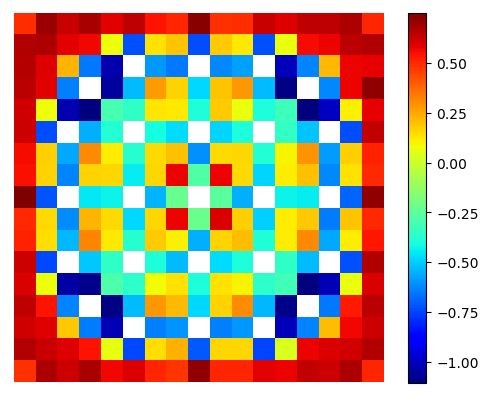
\includegraphics[width=\linewidth]{figures/assembly/capt-single-step-errors}
  \caption{}
  \label{fig:assm-capt-single-step-error}
\end{subfigure}%
\begin{subfigure}{0.45\textwidth}
  \centering
  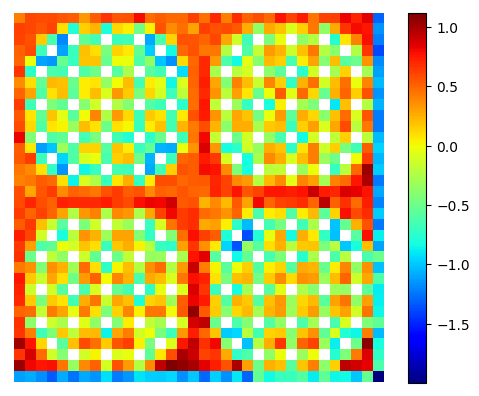
\includegraphics[width=\linewidth]{figures/colorset/capt-single-step-errors}
  \caption{}
  \label{fig:colorset-capt-single-step-error}
\end{subfigure}
\caption{OpenMOC U-238 capture rate percent relative errors for the assembly (a) and colorset (b) benchmarks.}
\label{fig:capt-errors}
\end{figure*}